%% ============================================================
%% Chapter 23: Expression Optimization
%% Algorithms for Optimization, 2nd ed. (2026)
%% Kochenderfer & Wheeler
%% ============================================================
\documentclass[aspectratio=169,10pt]{beamer}

\usetheme{Madrid}
\usecolortheme{seahorse}

\usepackage{amsmath,amssymb,amsfonts}
\usepackage{graphicx}
\usepackage{listings}
\usepackage{xcolor}
\usepackage{booktabs}
\usepackage{tikz}
\usetikzlibrary{trees,arrows.meta,positioning,shapes.geometric}
\usepackage{array}
\usepackage{multicol}
\usepackage{algorithm}
\usepackage{algpseudocode}

\graphicspath{{figures/}}

%% Python listing style
\lstdefinestyle{python}{
  language=Python,
  basicstyle=\ttfamily\scriptsize,
  keywordstyle=\color{blue!80!black}\bfseries,
  commentstyle=\color{gray!70}\itshape,
  stringstyle=\color{green!50!black},
  numberstyle=\tiny\color{gray},
  numbers=left,
  frame=single,
  backgroundcolor=\color{gray!7},
  breaklines=true,
  showstringspaces=false,
  tabsize=4,
  xleftmargin=1.5em,
  framexleftmargin=1.5em,
}

\setbeamertemplate{footline}[frame number]
\setbeamertemplate{navigation symbols}{}

%% ---- title page ----
\title[Ch.\ 23: Expression Optimization]{\textbf{Chapter 23: Expression Optimization}}
\subtitle{Algorithms for Optimization, 2nd Edition (2026)}
\author{Kochenderfer \& Wheeler}
\institute{Lecture Slides}
\date{}

% ===================================================================
\begin{document}
% ===================================================================

\begin{frame}
  \titlepage
\end{frame}

% -------------------------------------------------------------------
\begin{frame}{Chapter Outline}
  \tableofcontents
\end{frame}

% ===================================================================
\section{Motivation and Overview}
% ===================================================================

\begin{frame}{Why Expression Optimization?}
  \begin{columns}[T]
    \column{0.55\textwidth}
    \begin{block}{Key Idea}
      Optimize over \textbf{variable-size tree structures} (expressions,
      programs, formulas) instead of fixed-length vectors.
    \end{block}
    \bigskip
    \textbf{Applications:}
    \begin{itemize}
      \item Symbolic regression: discover equations from data
      \item Program synthesis: generate code to solve a task
      \item Design optimization: gear trains, circuits, robot controllers
      \item Feature engineering / model architecture search
    \end{itemize}
    \column{0.42\textwidth}
    \begin{exampleblock}{Core Challenge}
      The search space is \textbf{combinatorially large} and
      \textbf{variable-dimensional}; standard gradient methods
      do not apply. \\[4pt]
      We need representations that enforce
      \emph{syntactic correctness} automatically.
    \end{exampleblock}
  \end{columns}
\end{frame}

% ===================================================================
\section{23.1 Grammars (BNF, Context-Free)}
% ===================================================================

\begin{frame}{Grammars --- Definitions}
  \begin{block}{Context-Free Grammar (BNF)}
    A grammar $\mathcal{G}$ consists of:
    \begin{itemize}
      \item \textbf{Nonterminals} (types): symbols to be expanded, e.g.\ $\mathbb{R}$
      \item \textbf{Terminals}: leaf symbols, e.g.\ $x$, $2$, $+$
      \item \textbf{Production rules}: $\text{type} \mapsto \text{expansion}$
      \item \textbf{Start symbol}: the root type
    \end{itemize}
  \end{block}
  \medskip
  The symbol $|$ on the right-hand side means \emph{or} (alternative rules):
  \[
    \mathbb{A} \mapsto \text{rapidly} \mid \text{efficiently}
  \]
  is shorthand for two rules: $\mathbb{A}\mapsto\text{rapidly}$ and
  $\mathbb{A}\mapsto\text{efficiently}$.
\end{frame}

\begin{frame}{Grammar for Arithmetic Expressions}
  \begin{columns}[T]
    \column{0.48\textwidth}
    \begin{block}{Four-Function Calculator Grammar}
      \begin{align*}
        \mathbb{R} &\mapsto \mathbb{R} + \mathbb{R} \\
        \mathbb{R} &\mapsto x \\
        \mathbb{R} &\mapsto \ln(\mathbb{R}) \\
        \mathbb{R} &\mapsto 2
      \end{align*}
    \end{block}
    \textbf{Key properties:}
    \begin{itemize}
      \item $\mathbb{R}$ is the only nonterminal
      \item Terminals: $x,\,2,\,+,\,\ln$
      \item Every fully-expanded tree is a valid expression
    \end{itemize}
    \column{0.50\textwidth}
    \begin{figure}
      
\includegraphics[width=\linewidth]{fig_expression_tree.pdf}
      \caption{Derivation of $x + \ln(2)$ using the production rules}
    \end{figure}
  \end{columns}
\end{frame}

\begin{frame}{Grammar: Formal Structure}
  \begin{columns}[T]
    \column{0.52\textwidth}
    \begin{figure}
      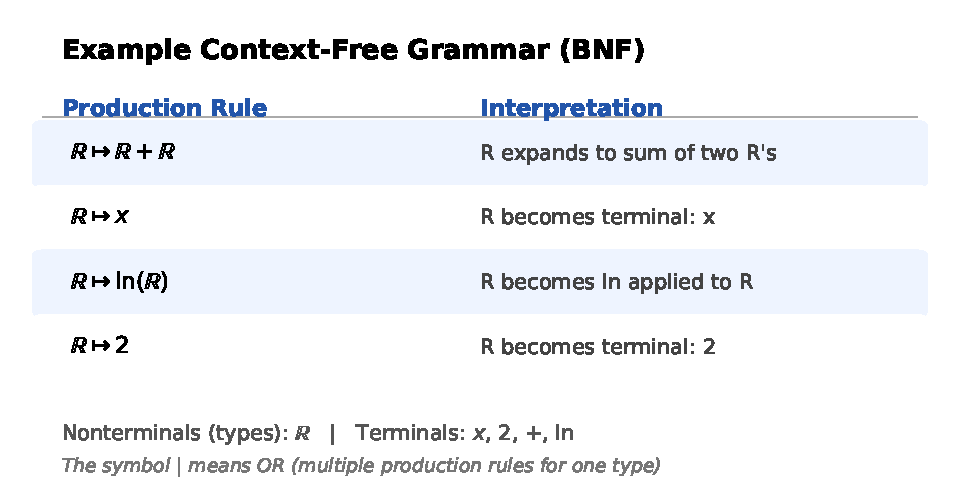
\includegraphics[width=\linewidth]{fig_grammar_bnf.pdf}
      \caption{BNF grammar: rules, nonterminals, and terminals}
    \end{figure}
    \column{0.45\textwidth}
    \begin{block}{English Grammar Example}
      \begin{align*}
        \mathbb{S} &\mapsto \mathbb{N}\,\mathbb{V} \\
        \mathbb{V} &\mapsto \mathbb{V}\,\mathbb{A} \\
        \mathbb{A} &\mapsto \text{rapidly} \mid \text{efficiently} \\
        \mathbb{N} &\mapsto \text{Alice} \mid \text{Bob} \mid \text{Mykel} \\
        \mathbb{V} &\mapsto \text{runs} \mid \text{reads} \mid \text{writes}
      \end{align*}
    \end{block}
    Derivation: $\mathbb{S}\!\to\!\mathbb{N}\,\mathbb{V}\!\to\!\text{Mykel}\,\mathbb{V}\,\mathbb{A}\!\to\!$ \textit{``Mykel writes rapidly''}
  \end{columns}
\end{frame}

\begin{frame}{Grammar Depth and Size}
  \begin{columns}[T]
    \column{0.55\textwidth}
    \begin{block}{Constraint: Maximum Depth}
      Expression optimization often constrains tree depth $d_{\max}$ to
      avoid infinite recursion or excessively large trees.
    \end{block}
    \medskip
    \begin{itemize}
      \item \textbf{Terminal node}: no children; a leaf of the tree
      \item \textbf{Nonterminal node}: an unexpanded type (blue nodes in figure)
      \item The number of expressions grows \emph{super-exponentially} with height $h$
      \item For $\mathbb{N}\mapsto\{\mathbb{N},\mathbb{N}\}\,|\,\{\mathbb{N},\}\,|\,\{,\mathbb{N}\}\,|\,\{\}$:
        \[ T(h) = 1 + 4 \cdot T(h-1)^2 \qquad (\text{super-exponential}) \]
    \end{itemize}
    \column{0.43\textwidth}
    \begin{exampleblock}{Four-Function Calculator (Example 23.2)}
      \vspace{2pt}
      Grammar (digits 1--9):
      \begin{align*}
        \mathbb{R} &\mapsto \{1,\ldots,9\} \\
        \mathbb{R} &\mapsto \mathbb{R} + \mathbb{R} \\
        \mathbb{R} &\mapsto \mathbb{R} - \mathbb{R} \\
        \mathbb{R} &\mapsto \mathbb{R} \times \mathbb{R} \\
        \mathbb{R} &\mapsto \mathbb{R} / \mathbb{R}
      \end{align*}
      An \textbf{infinite} number of expressions can be generated (no terminal constraint).
    \end{exampleblock}
  \end{columns}
\end{frame}

\begin{frame}[fragile]{Grammar Implementation in Python}
\begin{lstlisting}[style=python]
# Represent a grammar as a dict: type_name -> list of production rules
# Each rule is a tuple of (symbol, is_terminal) pairs

grammar = {
    "R": [
        # R -> R + R
        [("R","nt"), ("+","t"), ("R","nt")],
        # R -> x
        [("x","t")],
        # R -> ln(R)
        [("ln","t"), ("R","nt")],
        # R -> 2
        [("2","t")],
    ]
}

def is_terminal(symbol, grammar):
    return symbol not in grammar

def get_rules(symbol, grammar):
    return grammar.get(symbol, [])

# Random expression tree generation (depth-limited)
import random

def rand_tree(symbol, grammar, max_depth=5, depth=0):
    """Recursively build a random expression tree."""
    rules = get_rules(symbol, grammar)
    if not rules or depth >= max_depth:
        # Return a random terminal rule if forced
        term_rules = [r for r in rules if all(k=="t" for _,k in r)]
        rule = random.choice(term_rules if term_rules else rules)
    else:
        rule = random.choice(rules)
    children = []
    for sym, kind in rule:
        if kind == "nt":
            children.append(rand_tree(sym, grammar, max_depth, depth+1))
        else:
            children.append(sym)
    return (symbol, rule, children)

tree = rand_tree("R", grammar, max_depth=4)
\end{lstlisting}
\end{frame}

% ===================================================================
\section{23.2 Genetic Programming}
% ===================================================================

\begin{frame}{Genetic Programming --- Overview}
  \begin{columns}[T]
    \column{0.52\textwidth}
    \begin{block}{Key Idea}
      Apply genetic algorithms to \textbf{expression trees}. Populations of
      trees evolve via selection, crossover, and mutation.
    \end{block}
    \medskip
    \textbf{Algorithm Skeleton:}
    \begin{enumerate}
      \item Initialize population of random trees (grammar-constrained)
      \item Evaluate objective $f(\text{tree})$ for each individual
      \item Select parents (truncation, tournament, etc.)
      \item Apply \textbf{tree crossover} to produce offspring
      \item Apply \textbf{tree mutation} and/or \textbf{tree permutation}
      \item Repeat until convergence
    \end{enumerate}
    \column{0.45\textwidth}
    \begin{alertblock}{Key Difference from GA}
      Individuals are \textbf{variable-length trees}, not fixed-length
      vectors. Crossover and mutation must preserve type-correctness
      enforced by the grammar.
    \end{alertblock}
    \medskip
    \textbf{Reference:} Koza (1992); also used in symbolic regression
    (e.g.\ PySR, gplearn).
  \end{columns}
\end{frame}

\begin{frame}{Tree Crossover}
  \begin{columns}[T]
    \column{0.58\textwidth}
    \begin{figure}
      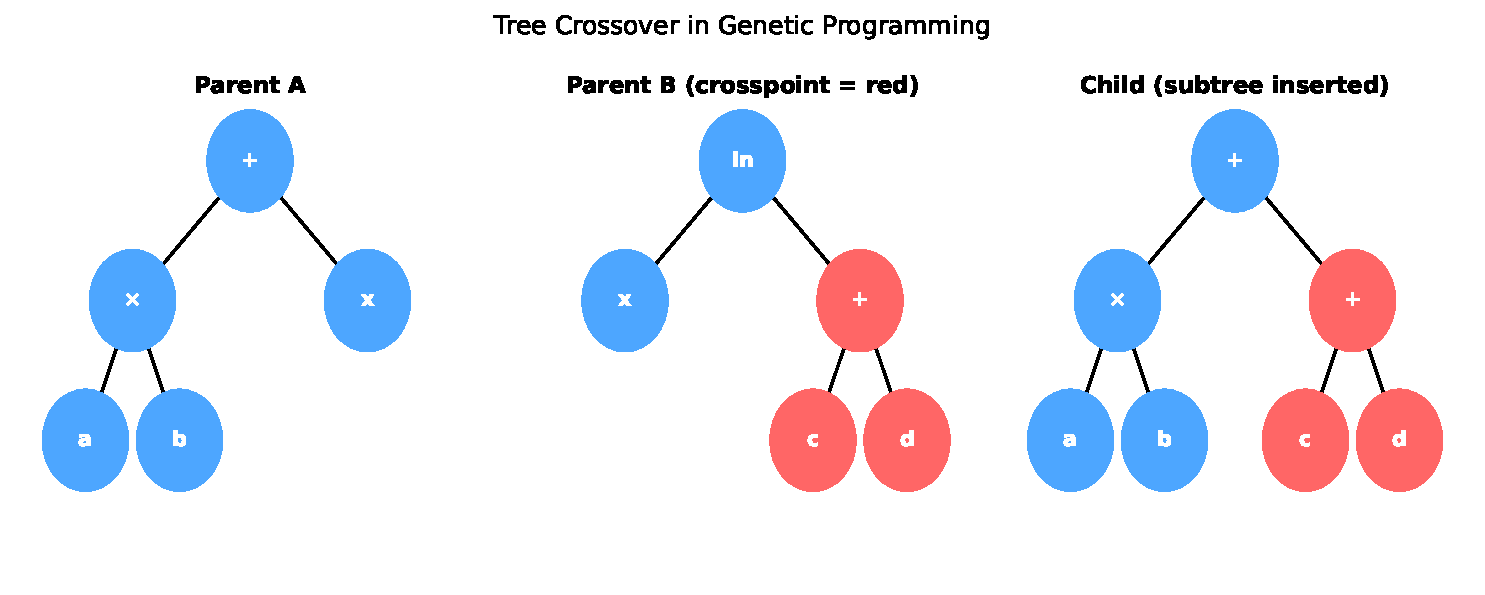
\includegraphics[width=\linewidth]{fig_tree_crossover.pdf}
      \caption{Tree crossover: a subtree from Parent B is inserted into Parent A at a type-compatible location.}
    \end{figure}
    \column{0.40\textwidth}
    \begin{block}{Algorithm 23.1 (Tree Crossover)}
      \begin{enumerate}\small
        \item Deep-copy parent $A$ as child
        \item Sample a random node (crosspoint) from $B$
        \item Get type of crosspoint in $B$
        \item Find compatible insertion location in child
        \item Insert deep-copy of crosspoint subtree
      \end{enumerate}
    \end{block}
    \medskip
    \textbf{Constraint:} Replacement nodes must have the
    \textbf{same return type}; only nodes within
    $d_{\max} - d_{\text{subtree}}$ depth are valid locations.
  \end{columns}
\end{frame}

\begin{frame}{Tree Mutation}
  \begin{columns}[T]
    \column{0.55\textwidth}
    \begin{figure}
      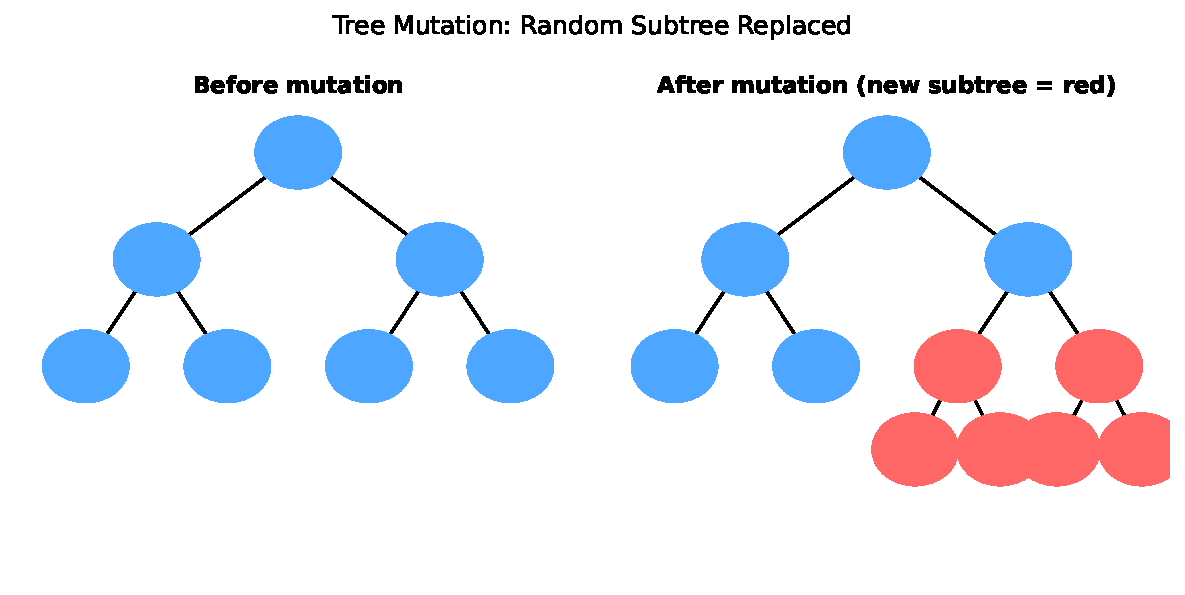
\includegraphics[width=\linewidth]{fig_tree_mutation.pdf}
      \caption{Tree mutation: a random subtree is deleted and replaced by a newly generated subtree of the same type.}
    \end{figure}
    \column{0.43\textwidth}
    \begin{block}{Algorithm 23.2 (Tree Mutation)}
      Given mutation probability $p$:
      \begin{enumerate}\small
        \item Deep-copy individual $a$
        \item With prob.\ $p$: sample random node location
        \item Get type at that location
        \item Generate new random subtree of same type
        \item Insert new subtree at location
      \end{enumerate}
    \end{block}
    Tree crossover tends to produce deeper trees; mutation
    introduces \textbf{new genetic material}.
  \end{columns}
\end{frame}

\begin{frame}{Tree Permutation}
  \begin{columns}[T]
    \column{0.55\textwidth}
    \begin{figure}
      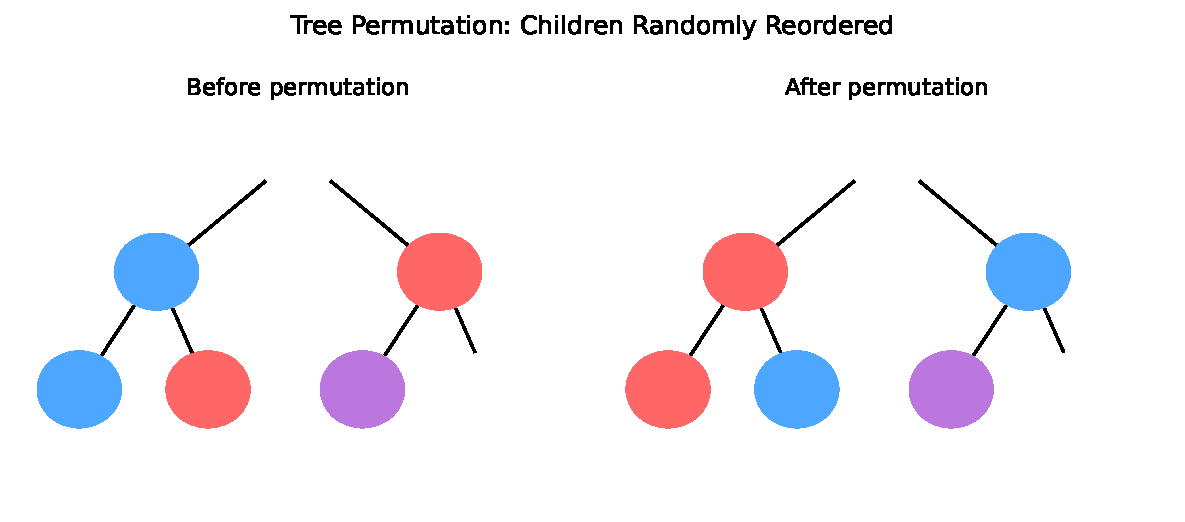
\includegraphics[width=\linewidth]{fig_tree_permutation.pdf}
      \caption{Tree permutation: children of a randomly chosen node are randomly reordered.}
    \end{figure}
    \column{0.43\textwidth}
    \begin{block}{Algorithm 23.3 (Tree Permutation)}
      Given mutation probability $p$:
      \begin{enumerate}\small
        \item Deep-copy individual $a$
        \item With prob.\ $p$: sample random node
        \item Count children $n$; get child types
        \item Use Fisher-Yates-style swap among type-compatible children
        \item Return permuted child
      \end{enumerate}
    \end{block}
    \medskip
    \textbf{Note:} Only children with \textbf{matching types} may be
    swapped. Often combined with tree mutation.
  \end{columns}
\end{frame}

\begin{frame}[fragile]{Genetic Programming: Python Implementation}
\begin{lstlisting}[style=python]
import random, copy, math
import numpy as np

# ---- Tree node representation ----
class Node:
    def __init__(self, rule, children=None):
        self.rule = rule          # production rule applied
        self.children = children or []

# ---- Tree crossover ----
def tree_crossover(parent_a, parent_b, grammar, max_depth=10):
    child = copy.deepcopy(parent_a)
    # Sample crosspoint from parent_b
    crosspoint = random_node(parent_b)
    typ = return_type(crosspoint, grammar)
    d_subtree = tree_depth(crosspoint)
    d_max = max_depth + 1 - d_subtree
    if d_max > 0:
        loc = find_location(child, grammar, typ, d_max)
        if loc is not None:
            insert(child, loc, copy.deepcopy(crosspoint))
    return child

# ---- Tree mutation ----
def tree_mutate(individual, grammar, p_mutate=0.1, max_depth=10):
    child = copy.deepcopy(individual)
    if random.random() < p_mutate:
        loc = random_node_loc(child)
        typ = return_type(get_node(child, loc), grammar)
        new_subtree = rand_tree(typ, grammar, max_depth)
        insert(child, loc, new_subtree)
    return child

# ---- Objective: approximate pi ----
def objective_pi(tree, grammar, lam=1e-3):
    value = eval_tree(tree, grammar)
    if math.isinf(value) or math.isnan(value):
        return float('inf')
    return math.log(abs(value - math.pi) + 1e-15) + lam * tree_size(tree)
\end{lstlisting}
\end{frame}

\begin{frame}[fragile]{Example 23.5: Approximating $\pi$ with Genetic Programming}
  \begin{columns}[T]
    \column{0.55\textwidth}
\begin{lstlisting}[style=python]
import math, random

# Grammar: digits 1-9 + arithmetic ops
grammar_pi = {
    "R": [
        [("R","nt"),("+","t"),("R","nt")],
        [("R","nt"),("-","t"),("R","nt")],
        [("R","nt"),("*","t"),("R","nt")],
        [("R","nt"),("/","t"),("R","nt")],
        # Terminals: digits 1-9
        *[[(str(d),"t")] for d in range(1,10)],
    ]
}

def objective(tree):
    val = eval_expr(tree)
    if not math.isfinite(val):
        return float('inf')
    delta = abs(val - math.pi)
    return math.log(delta + 1e-15) + len(tree)/1000

# Run genetic programming
pop_size, max_iter = 1000, 200
population = [rand_tree("R", grammar_pi, max_depth=10)
              for _ in range(pop_size)]
for gen in range(max_iter):
    scores = [objective(t) for t in population]
    # Truncation selection (top 50%)
    elite = sorted(zip(scores, population))[:pop_size//2]
    population = [t for _,t in elite]
    population += [tree_crossover(
        random.choice(population),
        random.choice(population),
        grammar_pi, max_depth=10)
        for _ in range(pop_size//2)]
best = min(population, key=objective)
# Best tree evaluates to ~3.141586 (matches pi to 4 d.p.)
\end{lstlisting}
    \column{0.43\textwidth}
    \begin{figure}
      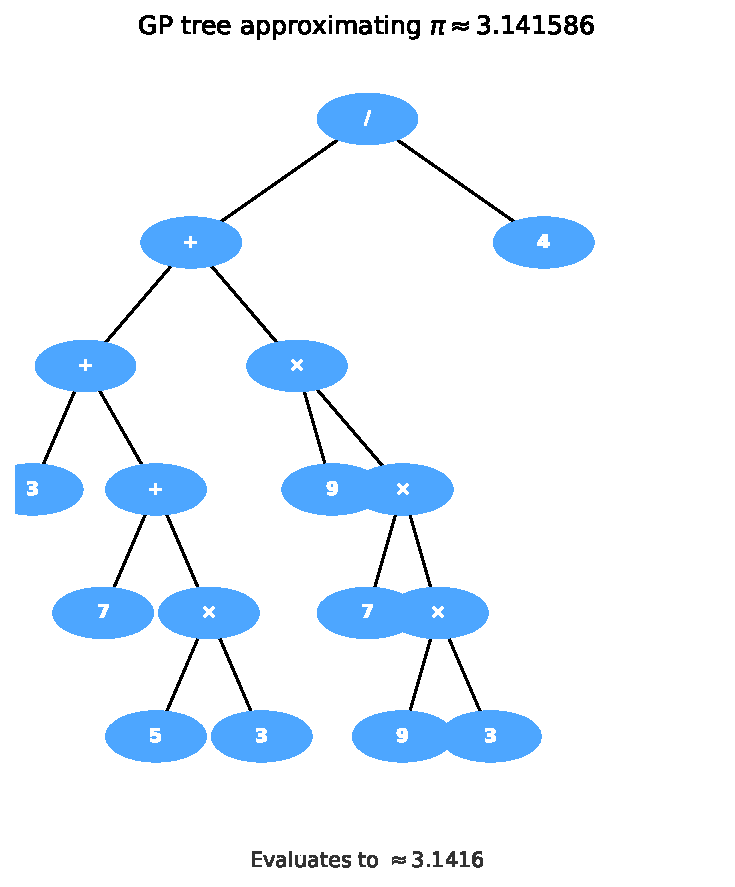
\includegraphics[width=0.85\linewidth]{fig_pi_tree.pdf}
      \caption{Best GP tree: evaluates to $\approx 3.141586$}
    \end{figure}
    \begin{exampleblock}{Result}
      Best performing tree evaluates to \textbf{3.141586},
      matching $\pi$ to four decimal places.
    \end{exampleblock}
  \end{columns}
\end{frame}

% ===================================================================
\section{23.3 Grammatical Evolution}
% ===================================================================

\begin{frame}{Grammatical Evolution --- Key Idea}
  \begin{columns}[T]
    \column{0.55\textwidth}
    \begin{block}{Integer Array Instead of Tree}
      Grammatical evolution operates on an \textbf{integer array} (chromosome)
      rather than directly on expression trees.
    \end{block}
    \medskip
    \textbf{Decoding Process:}
    \begin{enumerate}
      \item Start at root type
      \item At each nonterminal, use the next integer in the array to \textbf{select a production rule}
        \[ \text{rule index} = x[c] \bmod_1 |\text{rules}| \]
        (1-indexed modular arithmetic)
      \item Increment counter $c$; recurse on children
      \item Stop when all nonterminals are expanded or $c > c_{\max}$
    \end{enumerate}
    \column{0.43\textwidth}
    \begin{alertblock}{Advantages over GP}
      \begin{itemize}
        \item Standard GA operators (crossover, mutation) apply directly to integer arrays
        \item Grammar guarantees syntactic validity
        \item Integer representation is simpler to implement
      \end{itemize}
    \end{alertblock}
    \medskip
    \begin{exampleblock}{Key Parameters}
      $x$ = integer design vector \\
      $c_{\max}$ = max rule applications (prevents infinite loops)
    \end{exampleblock}
  \end{columns}
\end{frame}

\begin{frame}{Grammatical Evolution: Decoding (Algorithm 23.4)}
  \begin{columns}[T]
    \column{0.55\textwidth}
    \begin{block}{Algorithm: \texttt{decode}$(x,\,\mathcal{G},\,\text{sym},\,c_{\max})$}
      \begin{enumerate}\small
        \item $\text{types} \leftarrow \mathcal{G}[\text{sym}]$ \hfill (rules for type sym)
        \item If $|\text{types}| > 1$: $g \leftarrow x[c \bmod_1 |x|]$; $c \mathrel{+}= 1$
        \item $\text{rule} \leftarrow \text{types}[g \bmod_1 |\text{types}|]$
        \item $\text{node} \leftarrow \text{RuleNode}(\text{rule})$
        \item For each child type in rule (if $c < c_{\max}$): \\
              \quad recurse: $\text{cnode} \leftarrow $ \texttt{decode}$(x, \mathcal{G}, \text{ctyp}, c_{\max}, c)$
        \item Return \texttt{DecodedExpression}(node, $c$)
      \end{enumerate}
    \end{block}
    \column{0.43\textwidth}
    \begin{figure}
      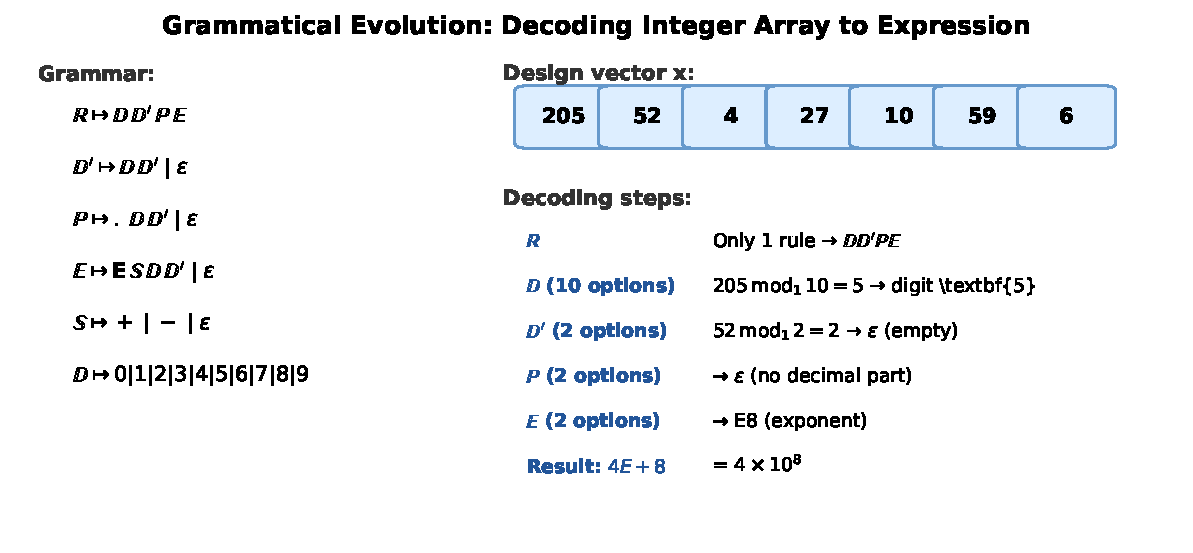
\includegraphics[width=\linewidth]{fig_grammatical_evolution.pdf}
      \caption{Decoding $[205,52,4,27,10,59,6]$ to expression $4E{+}8$}
    \end{figure}
  \end{columns}
\end{frame}

\begin{frame}{Grammatical Evolution: Worked Example}
  \begin{exampleblock}{Example 23.6: Real-Valued String Grammar}
    Grammar for real-valued numbers:
    \[
      \mathbb{R} \mapsto \mathbb{D}\,\mathbb{D}'\,\mathbb{P}\,\mathbb{E}, \quad
      \mathbb{D}' \mapsto \mathbb{D}\,\mathbb{D}' \mid \epsilon, \quad
      \mathbb{P} \mapsto .\,\mathbb{D}\,\mathbb{D}' \mid \epsilon
    \]
    \[
      \mathbb{E} \mapsto \mathbf{E}\,\mathbb{S}\,\mathbb{D}\,\mathbb{D}' \mid \epsilon, \quad
      \mathbb{S} \mapsto + \mid - \mid \epsilon, \quad
      \mathbb{D} \mapsto 0|1|2|3|4|5|6|7|8|9
    \]
  \end{exampleblock}

  \begin{columns}[T]
    \column{0.48\textwidth}
    \textbf{Design vector:} $[205, 52, 4, 27, 10, 59, 6]$
    \medskip
    \begin{tabular}{lll}
      \toprule
      Step & Choice & Result \\
      \midrule
      $\mathbb{R}$ & 1 rule only & $\mathbb{D}\mathbb{D}'\mathbb{P}\mathbb{E}$ \\
      $\mathbb{D}$ & $205 \bmod_1 10 = 5$ & digit \textbf{5} \\
      $\mathbb{D}'$ & $52 \bmod_1 2 = 2$ & $\epsilon$ \\
      $\mathbb{P}$ & choose $\epsilon$ & (no decimal) \\
      $\mathbb{E}$ & choose rule & $E+8$ \\
      \bottomrule
    \end{tabular}
    \column{0.48\textwidth}
    \textbf{Result:} String $= 4E{+}8 = 4\times10^8$
    \medskip
    \begin{alertblock}{Depth-First Decoding}
      The implementation is depth-first. If $52$ were instead $51$:
      $\mathbb{D}' \mapsto \mathbb{D}\,\mathbb{D}'$, eventually
      producing $43950.950E{+}8$.
    \end{alertblock}
  \end{columns}
\end{frame}

\begin{frame}[fragile]{Grammatical Evolution: Python Implementation}
\begin{lstlisting}[style=python]
import numpy as np

def decode(x, grammar, sym, c_max=1000, c=0):
    """
    Decode integer array x into an expression tree.
    x       : list/array of non-negative integers (chromosome)
    grammar : dict  type -> list of rules
    sym     : starting nonterminal symbol (str)
    c_max   : max rule applications (prevents infinite recursion)
    c       : current position counter (1-indexed modular)
    Returns : (node_dict, c)
    """
    rules = grammar[sym]
    if len(rules) > 1:
        g = x[(c % len(x))]   # 0-indexed Python
        c += 1
        rule = rules[g % len(rules)]
    else:
        rule = rules[0]

    node = {"sym": sym, "rule": rule, "children": []}
    child_types = [s for s, kind in rule if kind == "nt"]

    if child_types and c < c_max:
        for ctyp in child_types:
            cnode, c = decode(x, grammar, ctyp, c_max, c)
            node["children"].append(cnode)
    return node, c

# Crossover / mutation use standard numpy integer-array GA operators
def int_crossover(a, b):
    """Single-point crossover on integer chromosomes."""
    pt = np.random.randint(1, len(a))
    return np.concatenate([a[:pt], b[pt:]]), np.concatenate([b[:pt], a[pt:]])

def int_mutate(a, sigma=5):
    """Gaussian perturbation of integer chromosome."""
    return np.clip(a + np.random.randint(-sigma, sigma+1, size=len(a)), 0, 255)

# Duplication operator (GE-specific)
def duplicate(a):
    pt = np.random.randint(1, len(a))
    return np.concatenate([a, a[:pt]])
\end{lstlisting}
\end{frame}

\begin{frame}{GE Operators and Praxis}
  \begin{columns}[T]
    \column{0.55\textwidth}
    \textbf{Standard GA operators on the integer array:}
    \begin{itemize}
      \item \textbf{Crossover}: single-point or uniform on the integer chromosome
      \item \textbf{Mutation}: flip or add Gaussian noise to each integer
      \item \textbf{Duplication}: append a prefix of the chromosome to itself (inspired by gene duplication in DNA)
    \end{itemize}
    \medskip
    \begin{alertblock}{Drawbacks of Grammatical Evolution}
      \begin{enumerate}
        \item Hard to determine whether a chromosome encodes a valid/complete expression
        \item A small change in the chromosome can produce a \emph{large} change in the expression (locality problem)
      \end{enumerate}
    \end{alertblock}
    \column{0.43\textwidth}
    \begin{block}{Algorithm 23.5 (GE Crossover)}
      Single-point crossover on two integer arrays of type \texttt{GrammaticalEvolution}:
      \begin{enumerate}\small
        \item Sample crossover point
        \item Exchange tails
        \item Return two new chromosomes
      \end{enumerate}
    \end{block}
    \medskip
    \begin{block}{Algorithm 23.6 (GE Mutation)}
      For each element in the array, add random noise with probability~$p$.
    \end{block}
  \end{columns}
\end{frame}

% ===================================================================
\section{23.4 Probabilistic Grammars}
% ===================================================================

\begin{frame}{Probabilistic Grammars --- Motivation}
  \begin{columns}[T]
    \column{0.55\textwidth}
    \begin{block}{Idea: Learn Rule Selection Probabilities}
      Assign a \textbf{weight} $w_i^{\mathbb{T}}$ to each production rule $i$
      of type $\mathbb{T}$. The sampling probability is:
      \[
        P(\mathbb{T} \mapsto \text{rule}_i) = \frac{w_i^{\mathbb{T}}}{\sum_j w_j^{\mathbb{T}}}
      \]
    \end{block}
    \medskip
    \textbf{Optimization approach:}
    \begin{enumerate}
      \item Sample a population of expressions
      \item Evaluate and select elite samples
      \item \textbf{Update} the grammar weights based on elite rules used
      \item Iterate until convergence (similar to CEM / EDA)
    \end{enumerate}
    \column{0.43\textwidth}
    \begin{figure}
      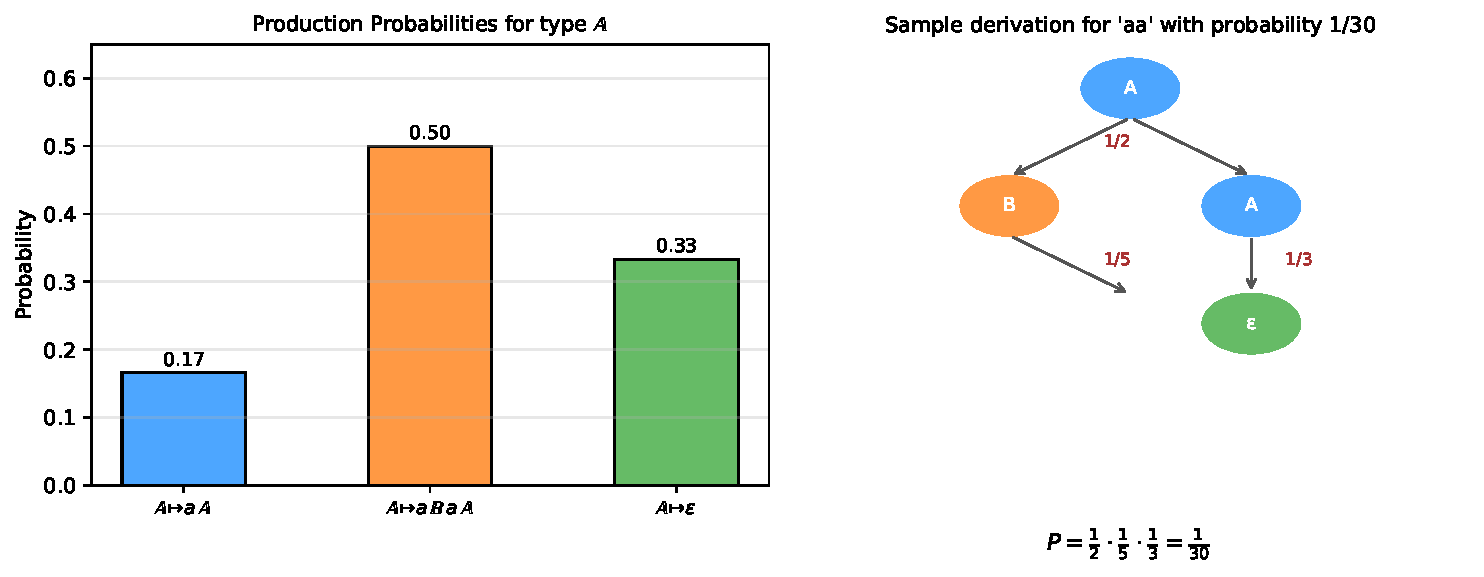
\includegraphics[width=\linewidth]{fig_probabilistic_grammar.pdf}
      \caption{Rule weights and sampling probabilities for a probabilistic grammar}
    \end{figure}
  \end{columns}
\end{frame}

\begin{frame}{Probabilistic Grammar: Likelihood and Update}
  \begin{exampleblock}{Example 23.7: Computing Expression Probability}
    Grammar for strings of ``a''s:
    \[
      \mathbb{A} \mapsto a\,\mathbb{A} \;(w=1), \quad
      \mathbb{A} \mapsto a\,\mathbb{B}\,a\,\mathbb{A} \;(w=3), \quad
      \mathbb{A} \mapsto \epsilon \;(w=2)
    \]
    \[
      \mathbb{B} \mapsto a\,\mathbb{B} \;(w=4), \quad
      \mathbb{B} \mapsto \epsilon \;(w=1)
    \]
    Sampling sequence for ``aa'':
    \[
      P(\mathbb{A}\!\mapsto\!a\,\mathbb{B}\,a\,\mathbb{A})\cdot P(\mathbb{B}\!\mapsto\!\epsilon)\cdot P(\mathbb{A}\!\mapsto\!\epsilon)
      = \frac{1}{2}\cdot\frac{1}{5}\cdot\frac{1}{3} = \frac{1}{30}
    \]
  \end{exampleblock}

  \begin{block}{Algorithm 23.10: Learning Update}
    Given an elite set of expressions $X_s$:
    \begin{enumerate}
      \item Reset all rule weights to 0
      \item For each expression $x \in X_s$: increment $w_i$ for every production rule $i$ used in $x$
      \item Result: weights reflect frequency of use in elite expressions
    \end{enumerate}
  \end{block}
\end{frame}

\begin{frame}[fragile]{Probabilistic Grammar: Python Code}
\begin{lstlisting}[style=python]
import numpy as np

class ProbGrammar:
    """Probabilistic context-free grammar with learnable weights."""
    def __init__(self, grammar):
        """
        grammar: dict  type -> list of rules (each rule is a list of (sym, kind))
        """
        self.grammar = grammar
        # Initialize weights uniformly
        self.weights = {typ: np.ones(len(rules))
                        for typ, rules in grammar.items()}

    def sample_rule(self, typ):
        """Sample a production rule index for type `typ`."""
        w = self.weights[typ]
        probs = w / w.sum()
        return np.random.choice(len(self.grammar[typ]), p=probs)

    def sample_expression(self, sym, max_depth=10, depth=0):
        """Recursively sample an expression tree."""
        rules = self.grammar[sym]
        if depth >= max_depth:
            # Force terminal rule
            term_idx = [i for i,r in enumerate(rules)
                        if all(k=="t" for _,k in r)]
            idx = np.random.choice(term_idx) if term_idx else 0
        else:
            idx = self.sample_rule(sym)
        rule = rules[idx]
        children = [self.sample_expression(s, max_depth, depth+1)
                    for s,k in rule if k=="nt"]
        return {"sym": sym, "rule_idx": idx, "children": children}

    def update_weights(self, elite_expressions):
        """Learning update: reset and count rule usage in elite set."""
        for typ in self.weights:
            self.weights[typ][:] = 0.0
        for expr in elite_expressions:
            self._count_rules(expr)

    def _count_rules(self, node):
        self.weights[node["sym"]][node["rule_idx"]] += 1
        for child in node["children"]:
            self._count_rules(child)
\end{lstlisting}
\end{frame}

% ===================================================================
\section{23.5 Probabilistic Prototype Trees}
% ===================================================================

\begin{frame}{Probabilistic Prototype Trees (PPT)}
  \begin{columns}[T]
    \column{0.55\textwidth}
    \begin{block}{Key Idea}
      A \textbf{probabilistic prototype tree} (PPT) stores a probability
      vector at \emph{every node} of the expression tree — one probability
      per applicable production rule at that position.
    \end{block}
    \medskip
    Unlike probabilistic grammars (which use \emph{global} rule probabilities),
    PPTs learn \textbf{position-specific} probabilities:
    \begin{itemize}
      \item Each node $\mathbf{p}_{ij\ldots}$ has its own probability vector
      \item The tree grows on demand when new positions are visited
      \item Probabilities are initialized uniformly; $w_{\text{terminal}}=0.6$, $w_{\text{nonterm}}=0.4$
    \end{itemize}
    \column{0.43\textwidth}
    \begin{figure}
      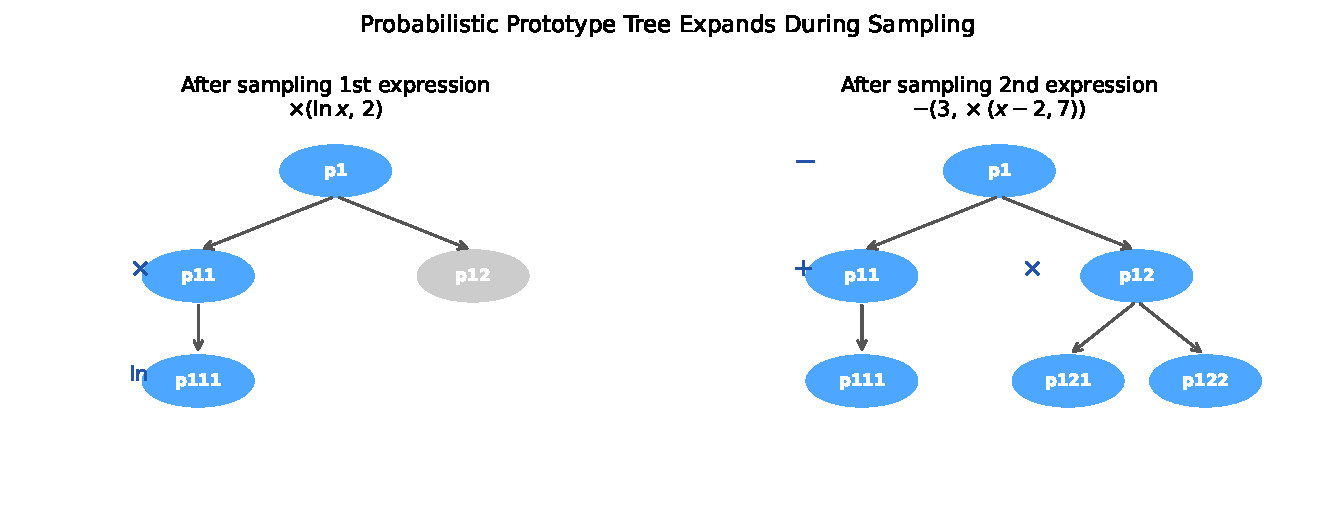
\includegraphics[width=\linewidth]{fig_ppt_growth.pdf}
      \caption{PPT expands as new expression positions are sampled}
    \end{figure}
  \end{columns}
\end{frame}

\begin{frame}{PPT: Sampling and Target Probability}
  \begin{columns}[T]
    \column{0.55\textwidth}
    \begin{block}{Target Probability (Algorithm 23.13)}
      Compute a target probability for the best-known expression:
      \[
        q_{\text{best}} = \left(\frac{1}{n_{\text{rules}}}\right)^{1/m}
      \]
      where $m$ is the number of components in $\mathbf{p}$ and
      $n_{\text{rules}}$ is the total number of rules applied to reach
      the best expression. \\[4pt]
      Larger $q_{\text{best}}$ $\Rightarrow$ bias toward top-performing solutions.
    \end{block}
    \column{0.43\textwidth}
    \begin{block}{Learning Update (Algorithm 23.14)}
      Iterative EDA-style:
      \begin{enumerate}\small
        \item Sample $m$ expressions from PPT
        \item Evaluate objective
        \item Find best expression $x_{\text{best}}$
        \item Update PPT toward $x_{\text{best}}$
        \item Prune irrelevant branches
        \item Repeat
      \end{enumerate}
    \end{block}
    \medskip
    \begin{exampleblock}{Equation (23.4)}
      \[
        f_{\text{target}}(x_s) = \prod_{k} q_{\text{best},k}^{n_k}
      \]
    \end{exampleblock}
  \end{columns}
\end{frame}

\begin{frame}{PPT: Mutation Update Rule}
  \begin{columns}[T]
    \column{0.55\textwidth}
    \begin{block}{Mutation Formula (Eq.\ 23.5)}
      For each component $p_i$ in a node's probability vector:
      \[
        p_i \;\mathrel{+}=\; \beta\,(1 - p_i)
      \]
      with probability $p_{\text{mutation}} / (\sqrt{|x_{\text{best}}|} \cdot \sqrt{m})$.
      Then \textbf{renormalize} the vector so it sums to 1.
    \end{block}
    \medskip
    \textbf{Interpretation:} Smaller probabilities receive
    \emph{larger} absolute increases (drives toward uniformity for
    non-selected entries), while selected entries are boosted.
    \column{0.43\textwidth}
    \begin{figure}
      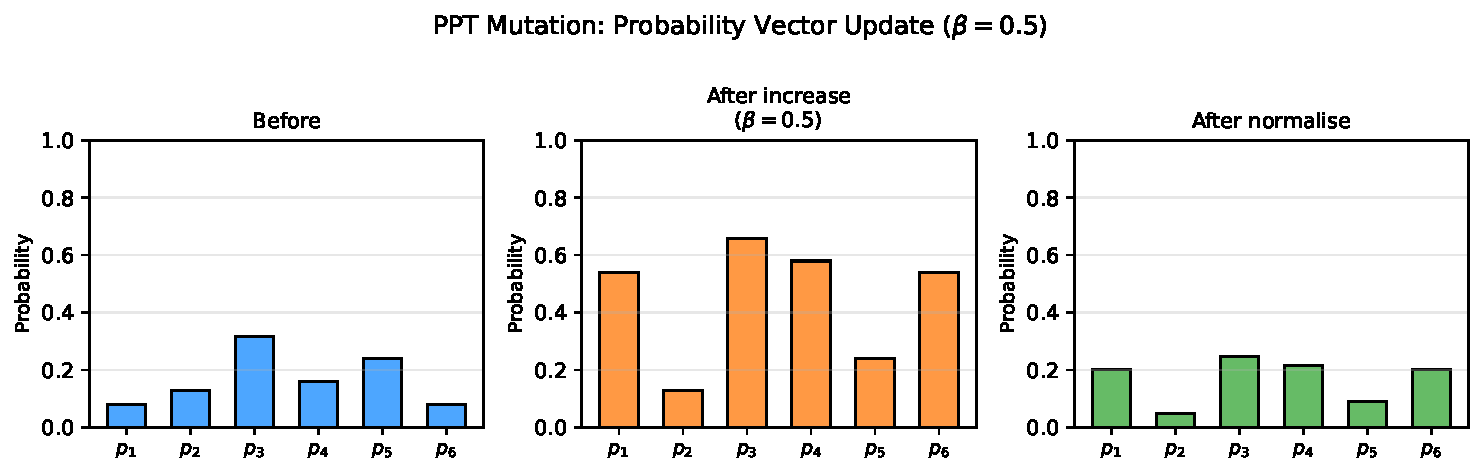
\includegraphics[width=\linewidth]{fig_ppt_mutation.pdf}
      \caption{Before / after increase / after normalize for $\beta=0.5$}
    \end{figure}
  \end{columns}
\end{frame}

\begin{frame}{PPT: Pruning (Algorithm 23.16)}
  \begin{columns}[T]
    \column{0.55\textwidth}
    \begin{block}{Pruning Condition}
      A PPT subtree can be \textbf{pruned} when the probability of its
      parent choosing a \emph{terminal} rule exceeds a threshold
      $p_{\text{threshold}}$ (typically 0.99):
      \[
        \max_i \, p_i^{(\text{parent})} > p_{\text{threshold}}
      \]
      If the dominant rule is terminal, children are unnecessary.
      If nonterminal, children with mismatched return type are pruned.
    \end{block}
    \column{0.43\textwidth}
    \begin{exampleblock}{Example 23.8: When to Prune}
      Node with rules:
      \begin{align*}
        \mathbb{R} &\mapsto \mathbb{R}+\mathbb{R} \\
        \mathbb{R} &\mapsto \ln(\mathbb{R}) \\
        \mathbb{R} &\mapsto 2 \mid x \\
        \mathbb{R} &\mapsto \mathbb{S}
      \end{align*}
      If $P(2)$ or $P(x)$ becomes large: children of that node become unnecessary and can be pruned.
    \end{exampleblock}
  \end{columns}
\end{frame}

\begin{frame}[fragile]{PPT: Python Implementation}
\begin{lstlisting}[style=python]
import numpy as np

class PPTNode:
    """Node in a Probabilistic Prototype Tree."""
    def __init__(self, grammar, w_terminal=0.6):
        self.grammar = grammar
        self.ps = {}  # type -> probability vector over rules
        self.children = []
        w_nonterm = 1.0 - w_terminal
        for typ, rules in grammar.items():
            ps_typ = np.array([w_terminal if is_terminal(grammar, i) else w_nonterm
                                for i, _ in enumerate(rules)], dtype=float)
            self.ps[typ] = ps_typ / ps_typ.sum()

    def get_child(self, i):
        """Lazily expand children as needed."""
        while len(self.children) <= i:
            self.children.append(PPTNode(self.grammar))
        return self.children[i]

def sample_from_ppt(ppt, grammar, sym):
    """Sample an expression tree from a PPT node."""
    rules = grammar[sym]
    rule_idx = np.random.choice(len(rules), p=ppt.ps[sym])
    rule = rules[rule_idx]
    child_syms = [s for s, k in rule if k == "nt"]
    node = {"sym": sym, "rule_idx": rule_idx, "children": []}
    for i, csym in enumerate(child_syms):
        child_ppt = ppt.get_child(i)
        node["children"].append(sample_from_ppt(child_ppt, grammar, csym))
    return node

def ppt_update(ppt, grammar, x_best, p_mutation=0.05, beta=0.5):
    """Update PPT probabilities toward x_best."""
    sqrtlen = np.sqrt(count_nodes(x_best))
    typ = x_best["sym"]
    p = ppt.ps[typ]
    prob = p_mutation / (len(p) * sqrtlen)
    for i in range(len(p)):
        if np.random.random() < prob:
            p[i] += beta * (1.0 - p[i])
    ppt.ps[typ] = p / p.sum()   # renormalize
    for ppt_child, x_child in zip(ppt.children, x_best["children"]):
        ppt_update(ppt_child, grammar, x_child, p_mutation, beta)
\end{lstlisting}
\end{frame}

\begin{frame}{Comparison: GP vs.\ GE vs.\ Prob.\ Grammar vs.\ PPT}
  \small
  \renewcommand{\arraystretch}{1.35}
  \begin{tabular}{lllll}
    \toprule
    & \textbf{GP} & \textbf{GE} & \textbf{Prob.\ Grammar} & \textbf{PPT} \\
    \midrule
    Representation     & Tree     & Integer array & Tree (+ weights)  & Tree (+ per-node weights) \\
    Grammar enforced   & Yes      & Yes           & Yes               & Yes \\
    Learns structure   & No       & No            & Global weights    & Position-specific \\
    Crossover          & Tree     & Integer       & N/A (EDA)         & N/A (EDA) \\
    Mutation           & Subtree  & Integer       & N/A               & Weight update \\
    Memory overhead    & Low      & Low           & Low               & High (tree grows) \\
    Locality           & Medium   & Poor          & Good              & Excellent \\
    \bottomrule
  \end{tabular}
  \medskip
  \begin{block}{Key Insight}
    PPTs trade \textbf{memory} for \textbf{locality}: every position in the expression
    tree has its own distribution, enabling fine-grained probability learning.
  \end{block}
\end{frame}

% ===================================================================
\section{23.6 Summary and Exercises}
% ===================================================================

\begin{frame}{Chapter 23 --- Summary}
  \begin{itemize}
    \item \textbf{Expression optimization} allows optimizing tree structures
      that, under a grammar, can represent sophisticated programs and designs
      lacking a fixed size.
    \medskip
    \item \textbf{Grammars} (BNF / context-free) define the production rules
      used to construct valid expressions; they guarantee syntactic correctness
      automatically.
    \medskip
    \item \textbf{Genetic programming} adapts genetic algorithms to perform
      mutation and crossover on expression trees (tree crossover, tree mutation,
      tree permutation).
    \medskip
    \item \textbf{Grammatical evolution} operates on an integer array that is
      decoded into an expression tree, enabling standard GA operators.
    \medskip
    \item \textbf{Probabilistic grammars} learn \emph{global} rule selection
      probabilities from elite expression samples.
    \medskip
    \item \textbf{Probabilistic prototype trees} learn \emph{position-specific}
      probabilities for every node in the expression tree via a mutation update rule.
  \end{itemize}
\end{frame}

\begin{frame}[allowframebreaks]{Selected Exercises}
  \begin{block}{Exercise 23.1}
    How many expression trees can be generated using the following grammar
    and starting set $\{\mathbb{R}, \mathbb{I}, \mathbb{F}\}$?
    \[
      \mathbb{R} \mapsto \mathbb{I} \mid \mathbb{F}, \quad
      \mathbb{I} \mapsto 1 \mid 2, \quad
      \mathbb{F} \mapsto \pi
    \]
    \textit{Solution:} Six trees: $\mathbb{I}\!\to\!1$, $\mathbb{I}\!\to\!2$,
    $\mathbb{F}\!\to\!\pi$, $\mathbb{R}\!\to\!\mathbb{I}\!\to\!1$,
    $\mathbb{R}\!\to\!\mathbb{I}\!\to\!2$, $\mathbb{R}\!\to\!\mathbb{F}\!\to\!\pi$.
  \end{block}

  \begin{block}{Exercise 23.2}
    The number of expression trees up to height $h$ grows super-exponentially.
    For $\mathbb{N}\mapsto\{\mathbb{N},\mathbb{N}\}\mid\{\mathbb{N},\}\mid\{,\mathbb{N}\}\mid\{\}$
    the count satisfies $T(h) = 1 + 4\,T(h-1)^2$, giving
    $T(1)=5$, $T(2)=101$, and so on.
  \end{block}

  \framebreak

  \begin{block}{Exercise 23.9: Probabilistic Grammar Likelihood}
    Grammar with weights:
    \begin{align*}
      \mathbb{R} &\mapsto \mathbb{R}+\mathbb{R}\mid\mathbb{R}\!\times\!\mathbb{R}\mid\mathbb{F}\mid\mathbb{I}
        & w_{\mathbb{R}} &= [1,1,5,5] \\
      \mathbb{F} &\mapsto 1.5 \mid \infty & w_{\mathbb{F}} &= [4,3] \\
      \mathbb{I} &\mapsto 1\mid 2\mid 3 & w_{\mathbb{I}} &= [1,1,1]
    \end{align*}
    Generation probability of $1.5 + 2$:
    \begin{align*}
      P(\mathbb{R}\!\mapsto\!\mathbb{R}+\mathbb{R}) &= 1/12, &
      P(\mathbb{R}\!\mapsto\!\mathbb{F}) &= 5/12 \\
      P(\mathbb{F}\!\mapsto\!1.5) &= 4/7, &
      P(\mathbb{R}\!\mapsto\!\mathbb{I}) &= 5/12 \\
      P(\mathbb{I}\!\mapsto\!2) &= 1/3
    \end{align*}
    \[
      P = \frac{1}{12}\cdot\frac{5}{12}\cdot\frac{4}{7}\cdot\frac{5}{12}\cdot\frac{1}{3}
        = \frac{25}{9072} \approx 0.00276
    \]
  \end{block}

  \framebreak

  \begin{block}{Exercise 23.8: Clock Gear Optimization}
    Design a gear train to produce second, minute, and hour hands.
    Objective (penalizes imprecision and tree complexity):
    \[
      \left(\min_{\text{hands}}\!(1-t_{\text{hand}})^2\right)
      + \left(\min_{\text{hands}}\!(60-t_{\text{hand}})^2\right)
      + \left(\min_{\text{hands}}\!(3600-t_{\text{hand}})^2\right)
      + \#\text{nodes}\cdot 10^{-3}
    \]
    Grammar (G$_r$ = gear of radius $r$, $\mathbb{R}$ = rim, $\mathbb{A}$ = axle, $\mathbb{H}$ = hand):
    \[
      G_r \mapsto \mathbb{R}\,\mathbb{A} \mid \epsilon, \quad
      \mathbb{R} \mapsto \mathbb{R}\,\mathbb{R} \mid G_r \mid \epsilon, \quad
      \mathbb{A} \mapsto \mathbb{A}\,\mathbb{A} \mid G_r \mid \mathbb{H} \mid \epsilon
    \]
    A minimal solution uses gears $G_{25}$, $G_{10}$, $G_{100}$ to
    produce rotation periods of $1$s, $60$s, and $3600$s.
  \end{block}
\end{frame}

\begin{frame}[fragile]{Exercise 23.8: Python Approach}
\begin{lstlisting}[style=python]
import numpy as np, math, random

# Grammar for gear train design
gear_grammar = {
    "G": [  # gear of some radius
        [("R","nt"), ("A","nt")],  # G -> rim + axle
        [],                         # G -> epsilon
    ],
    "R": [  # rim
        [("R","nt"), ("R","nt")],  # R -> R R
        [("G","nt")],               # R -> G
        [],                         # R -> epsilon
    ],
    "A": [  # axle
        [("A","nt"), ("A","nt")],  # A -> A A
        [("G","nt")],               # A -> G
        [("H","t")],                # A -> hand
        [],                         # A -> epsilon
    ],
}

def gear_objective(tree, radii):
    """
    Evaluate gear tree and compute period mismatch.
    radii: dict mapping gear_id -> radius
    """
    periods = get_hand_periods(tree, radii)
    if not periods:
        return float('inf')
    n_nodes = count_nodes(tree)
    targets = [1.0, 60.0, 3600.0]
    err = sum(min((p - t)**2 for t in targets) for p in periods)
    return err + n_nodes * 1e-3

# Solution: periods 1s, 60s, 3600s from G_25 -> G_10 -> G_100 chain
# G_25 drives G_10: ratio = 25/10 = 2.5  ... computed recursively
\end{lstlisting}
\end{frame}

% ===================================================================
% Final slide
% ===================================================================
\begin{frame}{Chapter 23: Key Takeaways}
  \begin{columns}[T]
    \column{0.48\textwidth}
    \textbf{What you should know:}
    \begin{enumerate}
      \item How to write a BNF grammar for a problem domain
      \item How GP crossover and mutation maintain type-correctness
      \item How GE decodes an integer array via modular indexing
      \item How probabilistic grammars update weights from elite samples
      \item How PPTs extend probabilistic grammars with per-node distributions
    \end{enumerate}
    \column{0.48\textwidth}
    \textbf{Connections to other chapters:}
    \begin{itemize}
      \item Ch.\ 9 (Genetic Algorithms): GP is GA applied to trees
      \item Ch.\ 9 (EDAs / CEM): probabilistic grammars and PPTs are EDAs over expression spaces
      \item Ch.\ 7 (Direct Methods): GE converts expression search to a standard real-valued search
    \end{itemize}
    \medskip
    \begin{block}{Take-Home Message}
      Grammars are the key: they enforce syntactic validity
      so that \textbf{every evaluated expression is legal},
      regardless of which optimization operator is applied.
    \end{block}
  \end{columns}
\end{frame}

\end{document}
